\documentclass[12pt, a4wide]{scrreprt}
\usepackage{scrhack}
\usepackage{scrpage2}
\usepackage{graphicx}
\usepackage[utf8]{inputenc}
\usepackage{ngerman}
\usepackage{multicol}
\usepackage[printonlyused,withpage]{acronym}
\usepackage{titlesec}
%numbers braucht man wohl für IEEEtranN
\usepackage[numbers]{natbib}

%irgendein hack für die Seitennummerierug-----v
\usepackage{tikzpagenodes}
\usetikzlibrary{calc}
\usepackage[contents={}]{background}
%--------------------------------------------^

\begin{document}
\setkomafont{disposition}{\normalcolor\bfseries}
%-------Titelseite-------%
\noindent
Konstantin Obermann \hfill Mat.nr: 947545\\
Universität Osnabrück \hfill 23.10.2015\\
Wintersemester 15/16\\
\thispagestyle{empty}
\begin{center}

\includegraphics[scale=.9]{uos_proper.png}
\section*{}
{\LARGE Ausarbeitung zum Thema}\\
\section*{}
{\Huge {\bf Lokalisierung in drahtlosen Sensornetzwerken}}\\
\section*{}
{\Large Im Rahmen des Seminars ''Verteilte Systeme''}\\
\section*{}
{\Large Betreuer:}\\
{\Large Prof.Dr.rer.nat Nils Aschenbruck}\\
{\Large Dipl.-Inform. Matthias Schwamborn}\\
\end{center}


\newpage
\thispagestyle{empty}
\section*{Abkürzungsverzeichnis}
 \begin{acronym}
\acro{WSN}{Wireless Sensor Network}
\acro{AOA}{Angle of Arrival}
\acro{RSS}{Received Signal Strength}
\acro{TOA}{Time of Arrival}
\acro{TDOA}{Time Difference of Arrival}
\acro{COTS}{Commercial Off-The-Shelf}
\end{acronym}

%-----------Inhaltsverzeichnis--------------%
\tableofcontents
\pagenumbering{roman}

\automark{chapter}
%-------Einleitung-------%
\chapter{Einleitung und Motivation}
%keine newpage bei neuem chapter
\renewcommand{\cleardoublepage}{}
\renewcommand{\clearpage}{}


\clearscrheadfoot
\pagestyle{scrheadings}
\ihead{\textnormal{Seite \thepage}}
\rohead{\headmark}
\setheadsepline{.1pt}
\renewcommand*{\chapterpagestyle}{scrheadings}

\pagenumbering{arabic}
Der technologische und wirtschaftliche Fortschritt erfordert eine zuverlässige, konsistente und in vielen Fällen drahtlose Kommunikation. Beispiele für drahtlose Netzwerke sind Mobilfunknetzstandards GSM, UMTS und LTE oder das drahtlose Netzwerkprotokoll WLAN.

Das \ac{WSN} dagegen ist ein Netz aus Sensoren. Die besondere Eigenschaft dieser Sensoren ist, dass sie sehr klein sind, auf kurze Distanzen miteinander kommunizieren, sowie Daten verarbeiten können und sparsam im Energieverbrauch sind. Sie können mithilfe ihrer Sensoren Informationen aus der Umwelt entnehmen und verarbeiten und besonders die Fähigkeit, ein Ad-hoc-Netz aufzuspannen, macht die \acs{WSN} zu einem vielfältig einsetzbaren drahtlosen Netzwerk.

Faktoren, wie Schnelligkeit und Präzision der Lokalisierung sowie der Grad der Autonomie des WSN, beeinflussen dessen Zuverlässigkeit und Potential. Dieses Potential ist entscheidend für die Auswahl der Einsatzmöglichkeiten. Das Erdbeben-Frühwarnsystem (EEW) ist eine der Anwendungsmöglichkeiten der \ac{WSN}. Hier ist eine reibungslose und schnelle Kommunikation zwischen den Knoten besonders wichtig, damit ein Ernstfall rechtzeitig erkannt werden kann. Weitere Beispiele für die Verwendung von Sensornetzen sind Erkennung von Waldbränden, Überwachung von Deichen, Überwachung von Gebäudestatik, um Erdbebenschäden zu erkennen\cite{building_monitoring} oder das ''Precision Farming''. Der Einsatz in Lagerhäusern bietet sich ebenfalls an, um ein- und auskommende Waren zu verwalten.

Diese Ausarbeitung beschäftigt sich mit Lokalisierungstechniken in \acs{WSN}. Zunächst werden in Kapitel 2 die Grundlagen der \acs{WSN} eingeführt, in Kapitel 3 Ansätze und zur Lokalisierung in diesen Netzwerken vorgestellt und in Kap.4 näher erläutert. Im 5.Kapitel werden Probleme behandelt, die bei der Lokalisierung auftreten können. Anschließend werden in Kap. 6 Beispiele für Anwendungsgebiete der \acs{WSN} vorgestellt.

\chapter{Wireless Sensor Network: Die Grundlagen}
Ein WSN besteht aus kleinen, vergleichsmäßig leistungsschwachen Sensoren, welche als Knoten (engl. nodes) im WSN dienen. Die Größe der Sensoren variiert je nach Ausstattung und Leistungsbedarf, überschreitet jedoch in der Regel nicht die Größe eines Schuhkartons. Die Kommunikation erfolgt auf dem Netzwerkprotokoll IEEE 802.15.4\footnote{Wireless Personal Area Networks Protokoll} oder auf dem \textit{ZigBee}, einer Erweiterung dieses Protokolls\cite{patwari_locating}.
Die Lebensdauer der Knoten reicht i.d.R. von 100-200 Stunden\cite{lifetime_study} bis zu 40 Jahren\cite{lisocl}.

Die eingeschränkte Leistung der Sensoren stellt eine Herausforderung beim Design des WSN dar. Um eine lange Betriebsdauer der Sensoren zu gewährleisten, ist eine exakt angepasste Hardware zu wählen, da zusätzliche Sensorik ebenso zusätzliche Auslastung und Energieverbrauch bedeutet, wobei Größe der Sensorknoten und somit ihre Arbeitsressourcen(RAM, CPU) nicht viel Spielraum für Rechenauslastung lassen.

Die bereits erwähnte Fähigkeit, automatisch ein Ad-hoc-Netz einzurichten, setzt voraus, dass sich die Knoten in einem Netzwerk selbstständig finden können und je nach Anwendungsgebiet entschieden werden muss, ob eine ungefähre Positionsbestimmung dieser Knoten ausreicht oder eine exakte Position ermittelt werden soll. Generell können bei der Auswahl der Lokalisierungsmethode folgende Faktoren als wichtig betrachtet werden: \textit{Genauigkeit}, \textit{Ausmaße des Anwendungsgebietes}, \textit{Kostenfaktor der Hardware}, \textit{Energieeffizienz} und \textit{Sicherheit der Software nach außen}\cite{indoor_localization}.

Die Lokalisierung der einzelnen Sensorknoten erfolgt auf Basis von auf Eintrittswinkel, Signalstärke oder der Distanz basierenden Ansätzen zur Positionsbestimmung. Zwar kann die Position der Knoten mit dem GPS ermittelt werden, allerdings erfordert die Vielseitigkeit der Einsatzmöglichkeiten der WSN eine Unabhängigkeit von der GPS-Positionierung, weil das GPS trotz der genauen Ortung ein zu schwaches Funksignal nutzt, um eine zuverlässige  Ortung innerhalb von Gebäuden oder unter der Erde möglich zu machen.

\chapter{Ansätze zur Positionsbestimmung}
Die Kombination aus Sensorhardware und Lokalisierungsmethode entscheidet über die Aufstellung der Knoten im \acs{WSN}. Abhängig von  Erreichbarkeit und Wartbarkeit der Sensoren in der Anwendung soll vor dem Einsatz des WSN die passende Hardware-Ausstattung geplant werden. Diese Ausstattung hängt von der gewählten Lokalisierungsmethode, aber auch vom Einsatzgebiet ab (Temperatur, Feuchtigkeit, Luftdruck).

Grundsätzlich unterscheidet man bei den Sensoren im WSN zwischen \textit{Anker} und \textit{nicht-Anker}. Die Ankerposition ist initial bekannt und die restlichen Knoten sollen ihre und die Position ihrer Nachbarn mithilfe der Anker bestimmen.

Diese Lokalisierungsansätze lassen sich in zwei grobe Kategorien einteilen\cite{area_based}: Die erste Kategorie umfasst die \textit{range-based} Methoden, welche mit Abstands- oder Winkelmessung arbeiten. Diese nutzen die im weiteren Verlauf beschriebenen Ansätze wie \ac{AOA}, \ac{RSS}, \ac{TOA} und \ac{TDOA}.

Die zweite Kategorie sind die \textit{range-free} Methoden, also Lokalisierungstechniken, die auf einen direkten Bezug zwischen den Sensorknoten verzichten, sondern nur Verbindungsinformationen nutzen. Diese sind zwar kostengünstiger und erfordern weniger komplexe Sensorik, sie sind aber nicht so präzise, wie die range-based Ansätze und werden in dieser Ausarbeitung nicht ausführlich behandelt. Eine der range-free Methoden ist die \textit{area-based}\cite{area_based} Lokalisierungstechnik. Das Prinzip hierbei ist, dass die Anker mithilfe von unterschiedlich empfangenen Signalstärken untereinander eine Fläche generieren, in welcher die Position des Senders geschätzt werden soll.

Die range-based Methoden eignen sich für WSNs, bei denen eine möglichst exakte Positionsbestimmung wichtig ist, wobei die Komplexität und somit die Kosten der Sensoren aufgrund des Bedarfes an Sensorik steigen. Range-free Lokalisierung ist eine Alternative, wenn die Ausstattung der Knoten im WSN möglichst kosteneffizient sein soll und die Kenntnis über die exakte Position der Sender nicht zwingend erforderlich ist.

\section{Hybride Lokalisierungsmethoden}
Zusätzlich zu den normalen Ansätzen werden immer mehr Lokalisierungsmethoden vorgeschlagen, die entweder unterschiedliche Ansätze miteinander verbinden\cite{rss-doa}, oder vorhandene Ansätze mit neuen Mitteln versehen, wie zum Beispiel die Nutzung eines RFID Chips als Identifikator für bestimmte Knoten im System\cite{rfid}. Oder die Nutzung einer Kamera, um die gemessene Distanz mit den aus Kamerabildern entnommenen Winkelinformationen zu verbinden, mit dem Ziel, genauere Ergebnisse zu erzielen\cite{range-video}.\\

Diese Ausarbeitung beschäftigt sich nicht mit den hybriden Ansätzen, dennoch sollte deren Existenz erwähnt sein. Im Folgenden werden die grundlegenden Ansätze zur Positionsbestimmung vorgestellt.

\chapter{Range-based Methoden}
  \section{Distanzbasierte Messung}
Im Folgenden werden Ansätze vorgestellt, welche den Abstand zwischen Sender und Empfänger ermitteln. Hierzu gehören \textit{Lighthouse approach}, \textit{\ac{TOA}}, \textit{Round-Trip Propagation} und \textit{\ac{TDOA}}.
    \subsection{Lighthouse Approach}
Das Verfahren, das dem \textit{Lighthouse approach}\cite{lighthouse} zugrunde liegt, basiert auf dem Prinzip eines Leuchtturms. Das Licht eines Lechtturms strahlt gerichtet und dreht sich um seine Achse, damit es von allen Seiten gesehen werden kann.\\
\indent
Für dieses Ortungsverfahren wird ein Sender benötigt, welcher als Leuchtturm fungiert. Die Empfänger des Signals müssen mit hoher Präzision arbeiten, also sollte das Licht des Senders ebenfalls möglichst ohne Abweichungen verlaufen. In {\bf Abb.3.2} ist der grobe Aufbau des \textit{Lighthouse approach} skizziert. Man kann erkennen, dass der Sender {\bf S} einen Strahl mit konstanter Breite {\bf b} ausstrahlt und sich um seine Achse dreht.\\

\begin{figure}[!htb]
\centering
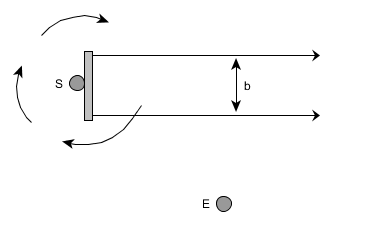
\includegraphics[scale=.68]{lighthouse.png}
\caption{Lighthouse Approach}
\end{figure}

Die Drehgeschwindigkeit des Senders ist vorher bekannt. Der Empfänger {\bf E} ist in Sichtweite aufgestellt und misst den Zeitunterschied zwischen dem Eintritt des Lichtsignals und dessen Austritt. Mithilfe der Drehgeschwindigkeit und der Zeit, die der Empfänger im Licht misst, kann die Entfernung berechnet werden.\\
\indent
Eine Möglichkeit, das Licht zu emittieren ist es, eine ausreichend breite parallele Lichtquelle zu nutzen. Parallel bedeutet, dass die Breite des Lichts unabhängig von der zurückgelegten Strecke möglichst konstant bleibt. Wie in \cite{lighthouse} beschrieben, ist dieses Vorgehen allerdings aufgrund von beschränkten Mitteln und Kapäzitäten der WSN Sensoren recht fehleranfällig und so wird z.B. ein 10cm breites Licht auf eine Entfernung von 5m eine Breite von 18.7cm erreichen.\\
\indent
Als Alternative ist es möglich, zwei Laser am Sender so anzubringen, dass sie einen in eine Richtung gerichteten, parallelen optischen Strahl simulieren. Mithilfe von vertikal und horizontal verstellbaren Spiegeln, an denen die Laser reflektiert werden, lassen sich feine Korrekturen an den Austrittswinkeln des Lichts vornehmen. Mit der \ac{COTS} Hardware lässt sich eine Drehfrequenz von bis zu 300Hz\cite{lighthouse} erreichen. 

    \subsection{One-Way Propagation}
\textit{One-Way Propagation} oder auch: \textit{\ac{TOA}} steht für die Übertragung eines Signals in eine Richtung\cite{toa}. Mithilfe der Übertragungszeit kann eine Distanz approximiert werden. Die Ausbreitungsgeschwindigkeit $c$\footnote{Lichtgeschwindigkeit} der Funkwellen ist bekannt. Diese Information lässt sich nutzen, um die Übertragungsdistanz zu errechnen. In der {\bf Abb. 3.3} sind 3 Anker und der Empfänger {\bf P} abgebildet. Die Radien aller 3 Anker schneiden sich in dem Punkt, an dem sich der Empfänger befinden soll.

\begin{figure}[!htb]
\centering
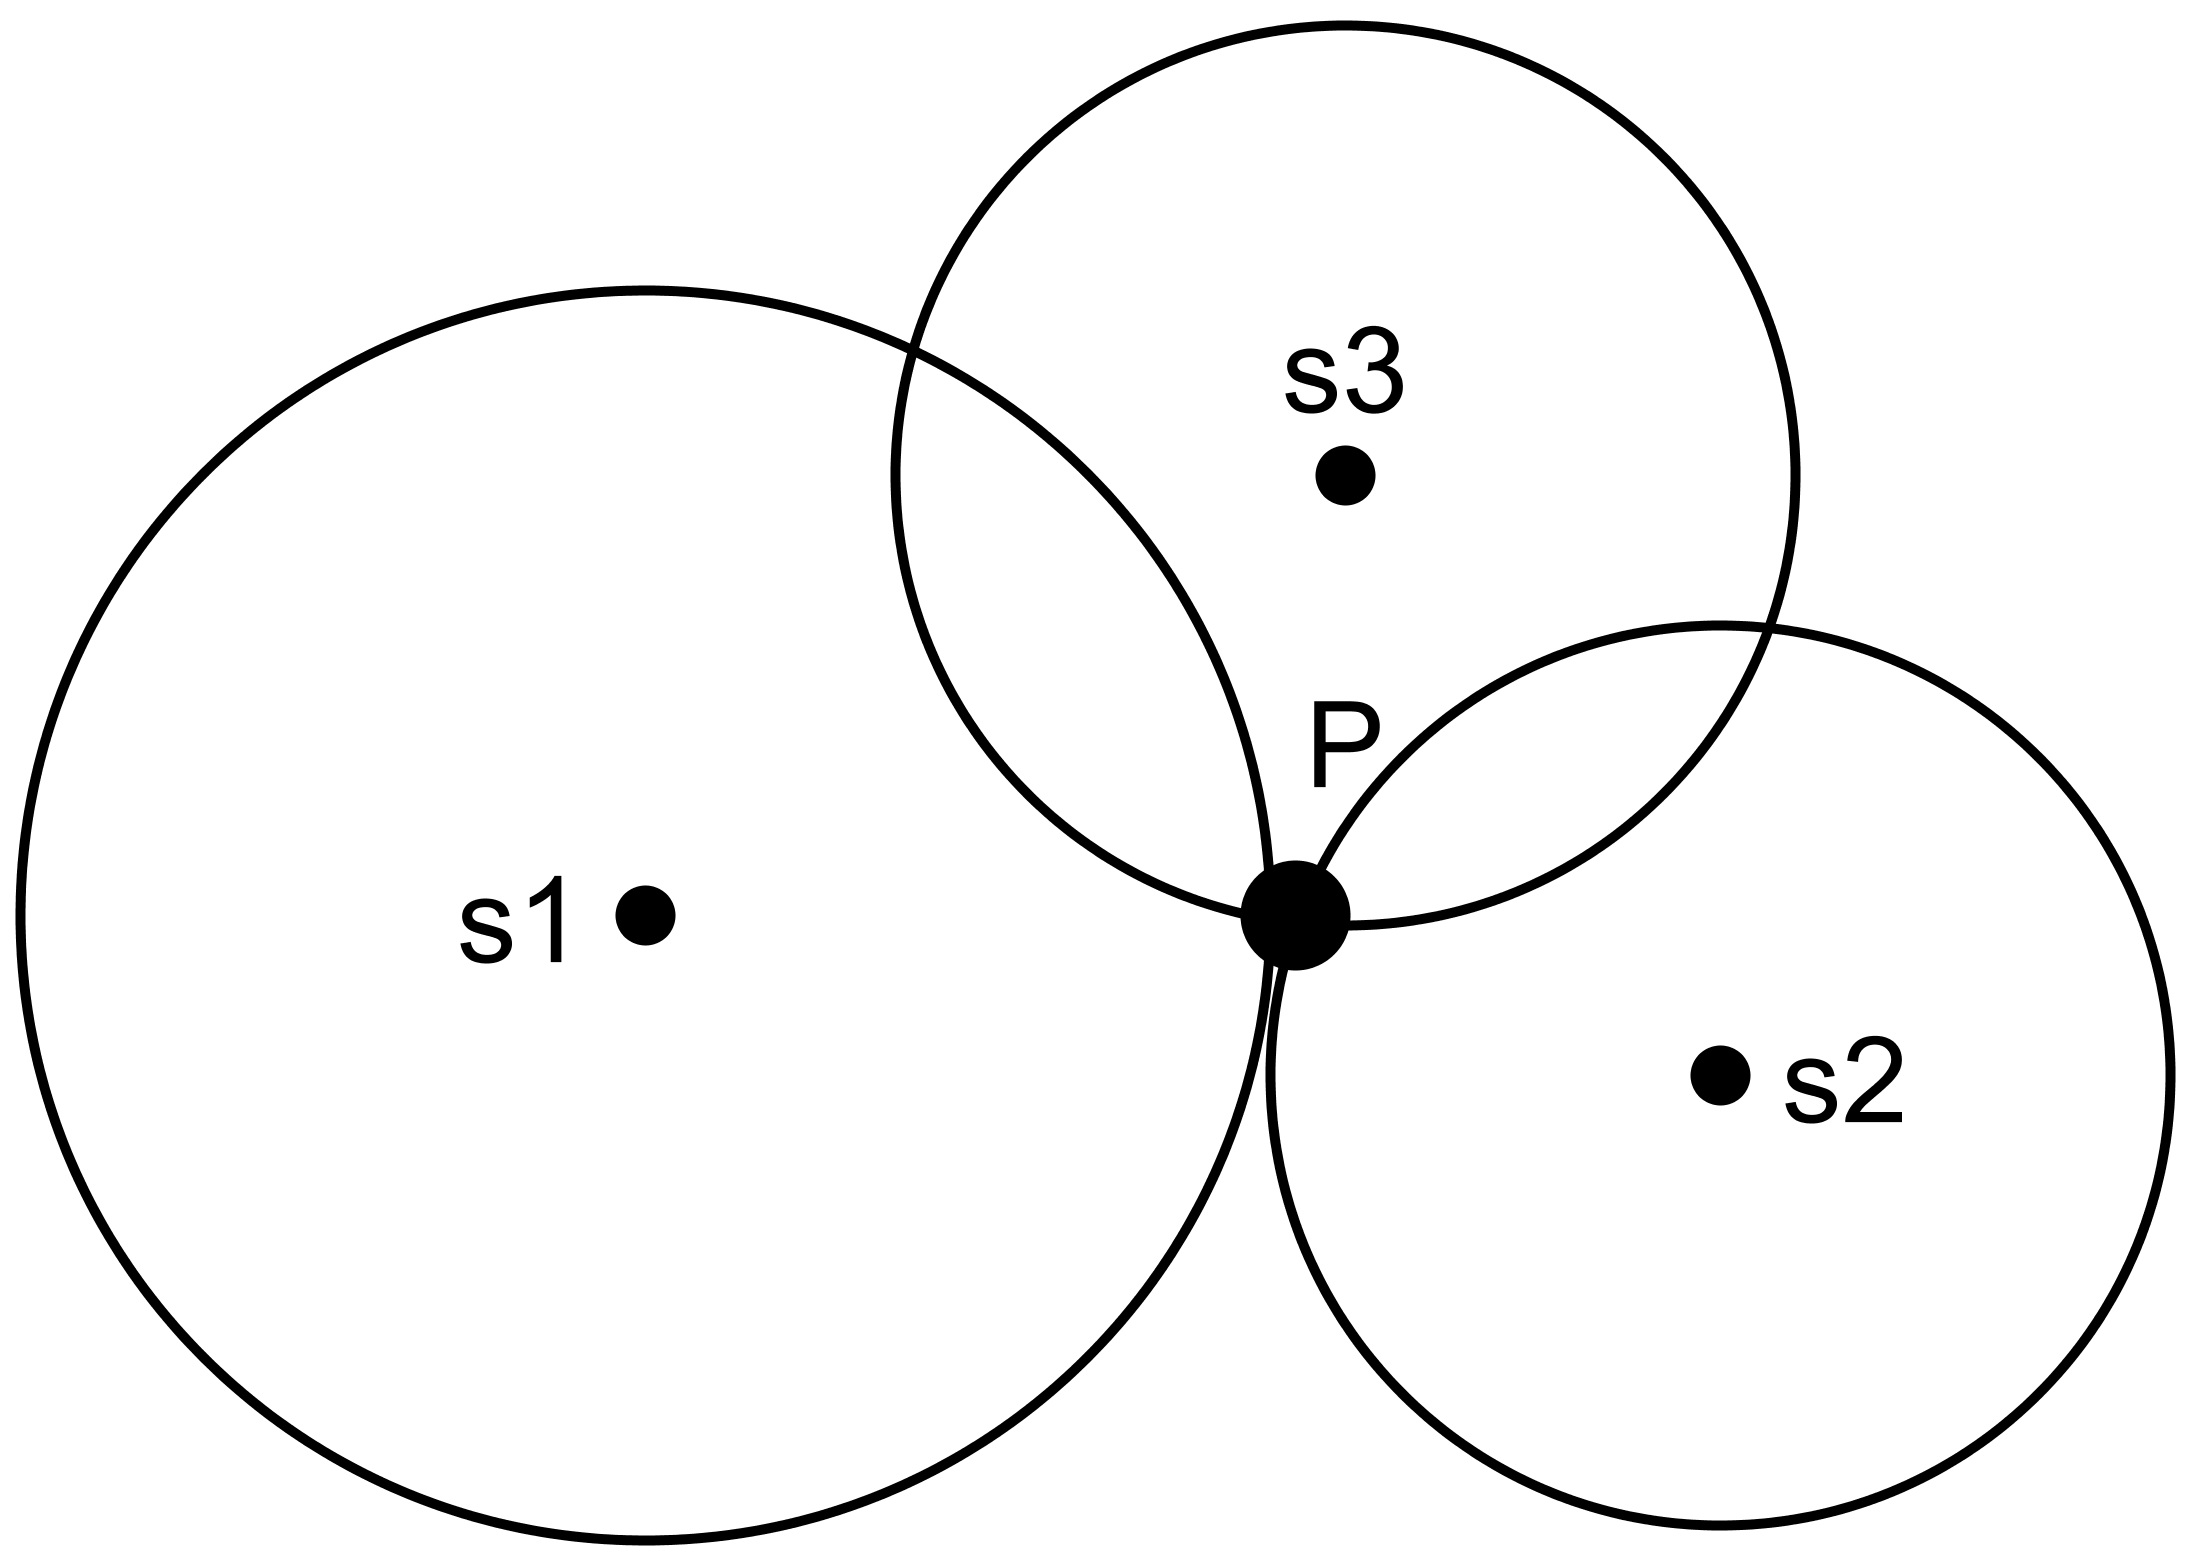
\includegraphics[scale=.07]{toa.png}
\caption{Zweidimensionale Lokalisierung mithilfe von TOA, Quelle:\cite{toa}}
\end{figure}

Man benötigt also mindestens 3 Anker, um die Position des Senders zu ermitteln. Der weitere wichtige Punkt ist die Synchronisierung der Geräte bezüglich der Uhren.
Um die Zeit zwischen dem Senden und Empfangen zu messen, muss der Empfänger die Uhrzeit des Sendens wissen. Die Uhr des Senders und die des Empfängers müssen also synchron laufen. Dies erfordert eine tiefere Kommunikation zwischen den Geräten, was die Komplexität der Hardware steigert. Das Vorgehen eignet sich also nicht besonders gut für \ac{WSN}, bei denen der Kostenfaktor minimal gehalten werden soll.

Eine mögliche Lösung zur Berechnung der Übertragungszeit wird in \cite{q1} erwähnt: Der Sender verschickt zusätzlich zum Radiosignal ein Ultraschallsignal. Das Radiosignal breitet sich mit $c$ aus und das Ultraschallsignal ist wesentlich langsamer. Der Empfänger horcht auf beide Signale und entsprechend der Differenz der Ankunftszeit kann die Übertragungsdauer berechnet werden. Allerdings steigt hierbei ebenfalls die Komplexität der Sensoren und das Vorgehen eignet sich nicht für Umgebungen mit ausgeprägtem potentiellen Mehrwegempfang. Mehr dazu in Kapitel 7. 

    \subsection{Time Difference Of Arrival}
Eine spezielle Abwandlung des \textit{\ac{TOA}}, welche mit Zeitdifferenzen eines ankommenden Signals arbeitet, ist die \textit{\ac{TDOA}}. Diese Methode erfordert auch eine Synchronisierung der Ankeruhren. Es werden 3 oder 4 Anker benötigt, deren Positionen bekannt sind. Diese dienen als Empfänger für das ankommende Signal des zu lokalisierenden Senders. Sobald das Signal an allen Ankern angekommen ist, wird die Zeitdifferenz für die Lokalisierung genutzt. Es ist zu beachten, dass die Präzision der Ortung steigt, wenn die Anker weiter voneinander entfernt platziert werden, sodass eine größere Zeitdifferenz beim Empfangen entsteht\cite{q1}. Es bietet sich an, einen für die zentrale Berechnung dedizierten Rechner zu stellen, welcher sowohl mit den Ankern, als auch mit den nicht-Ankerknoten kommuniziert und die daraus gewonnen Informationen für die Ortungsberechnung nutzt\cite{tdoa}.

    \subsection{Round-Trip Propagation}
Die erweiterte Alternative zur One-Way Propagation ist das \textit{Round-Trip} Prinzip, bei dem das Signal hin- und zurückgeschickt wird. Der Empfänger sendet das vom Anker empfangene Signal zurück, worauf der ursprüngliche Sender die Sende- und Rückkehrzeit seines Signals vergleichen kann. Anhand dieser Zeitdifferenz lässt sich dann die Distanz berechnen. Aus diesem Grund wird keine Synchronisierung der Sender- und Empfängeruhren benötigt. Abhängig von der Implementierung kann die Verarbeitungszeit zwischen dem Empfangen und Zurückschicken des Signals variieren. Eine mögliche Lösung ist es, dass der Empfänger diese Zeit selbst misst und an den Anker zusammen mit dem Empfangenen Signal zurück propagiert, damit die Abstandsberechnungen um diesen Zeitwert korrigiert werden können\cite{q1}.
    \subsection{RSS-basierte Entfernungsmessung}
Eine weitere Möglichkeit, zentralisierte Lokalisierungsberechnungen durchzuführen, ist die Bestimmung der Position mithilfe der empfangenen Signalstärke. Bei dieser Methode werden nicht nur Anker und nicht-Anker benötigt, sondern auch \textit{sniffing-devices}\cite{q1}. Diese werden über das Anwendungsgebiet verteilt und horchen auf die Signale der Anker in dem Gebiet, speichern die Informationen über die \ac{RSS} und anschließend werden diese Informationen an eine Zentrale weitergeleitet, die ein Abbild der Situation generieren soll. Die nicht-Anker sollen ihre Position anhand dieses Abbilds und der eigens empfangenen \ac{RSS} der Anker selbst einschätzen.

  \section{Angle Of Arrival Ansätze}
Das Prinzip der \acs{AOA} Lokalisierung ist es, den Eintrittswinkel des empfangenen Signals zu ermitteln. Dazu sollte der Empfänger einen ungehinderten Sichtkontakt zum Sender haben. Diese Lokalisierungsart kann in zwei Vorgehensweisen aufgeteilt werden: das \textit{Beamforming Prinpzip} und \textit{Phase Interferometry}. Generell erreichen die AOA Ansätze eine höhere Präzision, als mit den RSS Ansätzen auf Kosten von komplexerer Hardware\citep{q1}, wie z.B. Richtantennen.
    \subsection{Das Beamforming Prinzip}
Beim Beamforming wird mithilfe einer Richtantenne ein ankommendes Signal normiert, indem der Empfangskegel der Richtantenne mechanisch oder elektronisch gedreht wird, bis das empfangene Signal die höchste Sendeleistung erreicht. Somit kann die Richtung des Senders bestimmt werden. 

Bei diesem Vorgehen ist eine variierende Signalstärke das wichtigste Problem. Das Schwanken der Signalstärke führt zu einer falschen Wahrnehmung der Signalquellenrichtung. Ein Ansatz, welcher in \cite{q1} besprochen wird, befasst sich mit mehreren rotierbaren Richtantennen, deren gesammelte Informationen durch eine zentrale Einheit überlappt und ausgewertet werden, womit eine höhere Genauigkeit erreicht wird. So können mit 4 Richtantennen eine Richtungsgenauigkeit von $10^\circ -15^\circ$, mit 6 Antennen $5^\circ$ und mit bereits 8 Antennen eine Genauigkeit von $2^\circ$ erreicht werden\cite{q1}.
    \subsection{Phase Interferometry}
Mithilfe des \textit{phase interferometry}\cite{q1} Verfahrens lässt sich die Richtung eines eingehendes Signals durch eine Antennenfront(/-array) bestimmen. In {\bf Abb.3.1} ist der Aufbau skizziert. Hierbei sind $x1...xn$ die Antennen, alle mit dem gleichen, bekannten Abstand $d$ zueinander aufgebaut sind. Diese Antennen empfangen das Signal des Senders zu unterschiedlichen Zeitpunkten. Während die letzte Welle in diesem Beispiel gerade noch $x1$ verlässt, so tritt sie gleichzeitig bei $x2$ ein. Das ist der zeitliche Unterschied der empfangenen Phase, also die \textit{Phasenverschiebung}. Mithilfe dieses Phasenunterschiedes lässt sich mathematisch die Richtung des Senders bestimmen.\\

\begin{figure}[!htb]
\centering
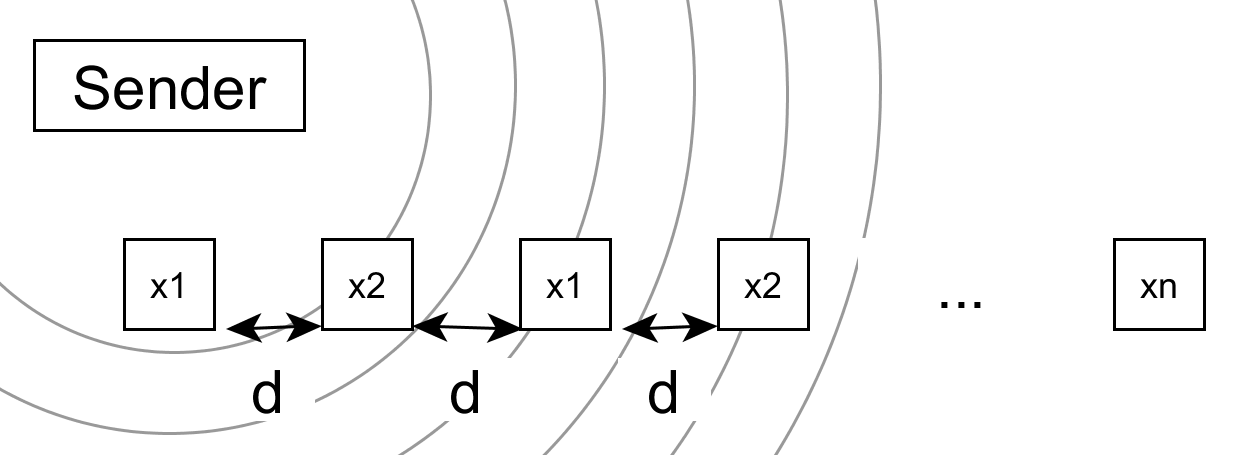
\includegraphics[scale=.27]{phase_int2.png}
\caption{Ankommende Wellenfronten an den Antennen}
\end{figure}

\section{Vergleich der Ansätze}
Jeder dieser Ansätze stellt eine gute Entfernungs- und Positionsschätzung dar. Die Präzision variiert jedoch und hängt zudem von Anzahl der Knoten und der Größe des Einsatzgebietes ab. In {\bf Abb. 4.4} ist der in \cite{patwari_locating} vorgestellte Vergleich der Lokalisierungseffizienz unter der Nutzung der erwähnten Ansätze. Man kann erkennen, dass die Fehleranfälligkeit, dargestellt in Metern, mit steigender Knotenanzahl sinkt. Das $r$ steht für den Messradius der Anker. $r = 10m$ bedeutet also, dass die Ankerknoten Messungen nur innerhalb eines Radiuses von $10m$ durchführen und $r = \infty$ bedeutet, dass alle Sensordaten erfasst werden.

\begin{figure}[!htb]
\centering
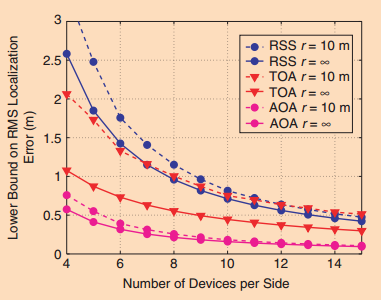
\includegraphics[scale=.6]{accuracy_patwari.png}
\caption{Präzision der Lokalisierung verschiedener Ansätze, Quelle:\cite{patwari_locating}}
\end{figure}

Unter explizit diesen Voraussetzungen\cite{patwari_locating} ist die AOA Methode präziser in der Lokalisierung anderer Knoten, als die anderen Methoden. Die Effizienz des RSS Ansatzes wächst jedoch mit steigenden Ankern schneller, als die der TOA Methode, obwohl diese mit einer geringen Anzahl an Ankern effizienter ist, als RSS.

Der Einsatz in unterschiedlichen Gebieten und unter anderen Voraussetzungen wird dieses Ergebnis sehr wahrscheinlich verändern, denn die Lokalisierungstechniken unterliegen mit unterschiedlicher Härte den Problemen, wie Mehrwegempfang oder Schwund des Signals. 

%\chapter{Range-free Methoden}
%http://delivery.acm.org/10.1145/940000/938995/p81-he.pdf?ip=131.173.191.68&id=938995&acc=ACTIVE%20SERVICE&key=2BA2C432AB83DA15%2E2BB856C4FB99BD06%2E4D4702B0C3E38B35%2E4D4702B0C3E38B35&CFID=735257829&CFTOKEN=37434624&__acm__=1449160971_7742a273b04a36ba04a573683866b02a
%    \section{Flächenbasierte Lokalisierung}
%Die flächenbasierte Lokalisierung ist eine Spezialform der \textit{range-free} Lokalisierungsansätze.
\chapter{Probleme und Fragestellungen}
  \section{Auftretende Messfehler}
\textit{Multipath propagation}(Mehrwegempfang) ist eines der Störfaktoren in der drahtlosen Übertragung. Die Eigenschaft der Funkwellen ist, dass diese sich nicht in eine Richtung, sondern konzentrisch in alle Richtungen ausbreiten. Diese Wellen werden an fast allen Oberflächen (Gebäude, Hügel, Wasser) reflektiert. In der {\bf Abb 6.1} ist das von A emittierte Signal abgebildet, welches bei B unter unterschiedlichen Winkeln, und auch zu unterschiedlichen Zeiten, eintrifft. Dies kann dafür sorgen, dass das Signal durch die Interferenz der Signale, die phasenverschoben sind, stark geschwächt wird. Außerdem können diese reflektierten Signale nicht ohne Weiteres dem Ursprungssignal zugeordnet werden, was in der Regel zu einer fälschlicherweise interpretierter neuer, oder mehreren, Signalquelle(n) führen kann.

\begin{figure}[!htb]
\centering
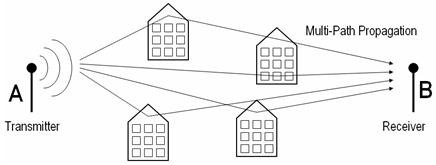
\includegraphics[scale=1]{multipath.png}
\caption{Reflektion des Radiosignals, Quelle:\cite{multipath}}
\end{figure}

  \section{Algorithmen zur Behebung von Messfehlern}
Die Effekte des multipath und des shadowing lassen sich mit dem Einsatz richtiger Algorithmen und Vorgehen korrigieren. Zum Beispiel kann der längere Einsatz der RSS Messung und die anschließende Mittelwertbildung der Signalstärke die Ungenauigkeiten eliminieren\cite{gezici2008survey}. Eine weitere Möglichkeit ist der Einsatz von sog. \textit{maximum-likelihood} Algorithmen\cite{q1}. Diese erfordern komplexe Berechnungen, können jedoch alle (inklusive reflektierter) Signale erfassen und die tatsächliche Quelle approximieren.

Bei den distanzbasierten Ansätzen gibt es die Möglichkeit, das kommerziell erwerbliche Ultrabreitband (UWB) zu nutzen\cite{q1}, dessen hohe Bandbreite von mehr als $500MHz$ es ermöglicht, kurze Impulse zu senden, die nicht so anfällig für Mehrwegempfang sind.

TODO

\section{Offene Fragen}
Neben den Messproblemen stellt das Design des WSN eine offene Problematik dar. Neben der Kosten- und Energieverbrauchsminimierung stellt die Auswahl des Netzwerkprotokolls eine weitere Herausforderung dar. Die am weitesten verbreitete Standards für die WSN sind IEEE 802.15. und das erweiterte ZigBee\cite{patwari_locating}. Ein weiterer offener Punkt in der Forschung ist die Entwicklung einer modularen und wartbaren Dienstschicht der WSNs\cite{issues_wsn}, die u.a. den Energieverbrauch durch Optimierung der Hardwarekommunikation senkt.
\chapter{Einsatzmöglichkeiten}
Die Einsatzmöglichkeiten der WSN umfassen viele Bereiche. Eines davon ist das in \cite{zebranet} vorgestellte \textit{ZebraNet}, dessen Zweck es ist, das Verhalten von Wildtieren zu beobachten. Da in einem nicht besiedelten Gebiet in der Regel keine Funkzellen vorhanden sind und eine GPS Lokalisierung zu teuer und zu energieverbrauchend ist, eignet sich hierfür ein WSN sehr gut. Die Tiere werden mit Halsbändern ausgestattet, in denen jeweils ein WSN Knoten mit eigener CPU und einem Very High Frequency(VHF) Sender/Empfänger verbaut ist. Diese Knoten sollen untereinander kommunizieren und die Informationen über die Bewegungen sammeln. ZebraNet wurde so entwickelt, dass keine gebundene Basisstation nötig ist, sodass die Anwender mithilfe von mehreren mit Sensoren ausgestatteten Fahrzeugen mobile Anker bilden und mithilfe von Triangulation die Sensoren der Tiere auslesen können. Aufgrund des Verzichtes auf das GPS kann eine Lebensdauer von bis zu einem Jahr erwartet werden. 

In der Einleitung wurde das ''precision farming'' erwähnt. Hierbei werden Sensorknoten auf einem landwirtschaftlich genutzten Feld verteilt, damit sie die Luftfeuchtigkeit, Temperatur und Grundwasserspiegel oder die Beschaffenheit des Bodens messen können. Diese Information sollen ausgewertet und die Produktivität der Ernte steigern. Zusätzlich können WSN in Gewächshäusern\cite{horticulture} platziert und für die Überwachung von Obst-/ Gemüsewachstum genutzt werden. In dieser Anwendung wird keine exakte Ortung der Sensoren benötigt. Es kann also auf teure Hardware verzichtet werden.

Eine weitere Möglichkeit, WSNs sinnvoll einzusetzen, ist die Überwachung von Bauwerken. Diese können einsturzgefährdete historische Gebäude sein\cite{historical_monitoring} oder große ausgelastete Brücken wie die Golden Gate Bridge\cite{bridge_monitoring}, deren strukturelle Reaktionen auf Vibrationen festgestellt und darauf basierend Tendenzen der Schwachstellen erstellt werden. Es können auch Analysen von Erdbebenschäden mithilfe von angebrachten Sensoren durchgeführt werden. Beim Anbringen der Sensoren an Gebäuden ist zu beachten, dass nicht alle Sensoren eine direkte Sichtlinie zu anderen Knoten im WSN haben können. Hierfür eignen sich die AOA Ansätze nicht besonders gut, da diese sich die Berechnungen auf die Sichtlinie zwischen Sensoren verlassen.

\chapter{Zusammenfassung}
Diese Ausarbeitung stellte in den ersten beiden Kapiteln die Wireless Sensor Networks und deren Besonderheiten vor und welche Herausforderungen sich in der Praxis ergeben. Hauptsächlich beschäftigte sich die Ausarbeitung mit den grundlegenden range-based Lokalisierungsmethoden AOA, TOA, TDOA, RSS und wie sie in den WSNs eingesetzt werden können.
\newpage
\bibliographystyle{IEEEtranN}
\bibliography{sources}
\nocite{*}
\end{document}